%! Author = Metougui Taha
%! Date = 26/02/2022

% Preamble
\documentclass[11pt]{article}

\usepackage{graphicx}
\usepackage{geometry}
\usepackage[utf8]{inputenc}
\usepackage[T1]{fontenc}
\usepackage[hidelinks]{hyperref}
\usepackage{fancyhdr}
\usepackage{amsmath}

\renewcommand{\abstractname}{\Large{Acknowledgements}}

% Document
\begin{document}

    \thispagestyle{empty}

    \begin{titlepage}
        \begin{center}
            
\includegraphics[width=150px]{images/logoEnsa}

            \vspace*{2cm}

            \Large
            \textbf{Implementation of industrial standards on a SaaS for an MVP for logistics}

            \vspace{0.5cm}
            \large
            \textbf{Metougui Taha}

            \vspace{1.5 cm}

            \textbf{Supervised by:}\\
            \vspace{0.5cm}
            \textbf{Pr. Zineb BESRI}\\
            \vspace{0.5cm}
            \textbf{Mr. Othman DARRAZ}

            \vspace{0.8 cm}
        \end{center}
    \end{titlepage}

    \newpage

    \begin{abstract}

    \end{abstract}

    \newpage

    \section{Acronyms}\label{sec:acronyms}
    \begin{table}[!htpb]
    \centering
    \begin{tabular}{| c | c |}
        \hline
        API & Application Programming Interface\\
        \hline
        AWS & Amazon Web Services\\
        \hline
        App & Application\\
        \hline
        CD  & Continuous Delivery\\
        \hline
        CEO & Chief Executive Officer\\
        \hline
        CI  & Continuous Integration\\
        \hline
        CLI & Command Line Interface\\
        \hline
        CTO & Chief Technology Officer\\
        \hline
        DB   & Database\\
        \hline
        DDOS & Distributed Denial of Service\\
        \hline
        ECR  & Elastic Container Registry\\
        \hline
        ECS  & Elastic Container Service\\
        \hline
        HTTP & Hypertext Transfer Protocol\\
        \hline
        IP   & Internet Protocol address\\
        \hline
        IT   & Information Technology\\
        \hline
        JS   & JavaScript\\
        \hline
        JVM  & Java Virtual Machine\\
        \hline
        JWT  & JSON Web Token\\
        \hline
        KPI  & Key performance indicator\\
        \hline
        MQTT & Message Queuing Telemetry Transport Protocol\\
        \hline
        MVP  & Minimum viable product\\
        \hline
        OAuth & Open Authentication Protocol\\
        \hline
        OOP  & Object Oriented Programming\\
        \hline
        PoC  & Proof of concept\\
        \hline
        RATP & Régie autonome des transports parisiens\\
        \hline
        RDS  & Relational Database Service\\
        \hline
        REST & Representational State Transfer\\
        \hline
        S3   & Simple Storage Service\\
        \hline
        SCM  & Supply Chain Management\\
        \hline
        SCP & Secure Copy\\
        \hline
        SOA  & Service Oriented Architecture\\
        \hline
        SSH & Secure Shell\\
        \hline
        SSM  & Secrets Management\\
        \hline
        SaaS & Software as a service\\
        \hline
        VPS  & Virtual Private Server\\
        \hline
    \end{tabular}
\end{table}


    \newpage

    \tableofcontents

    \newpage

    \section{Introduction}\label{sec:introduction}
    At the growth rate multiple industries are going through, it's no secret that the reliance
on automated and self-sustaining systems is increasing especially in the fields of
logistics, finance, and manufacturing. Targeting more specifically the supply chain
logistics, the industry is looking for solutions that can automate decision making
processes of moving goods from one place to another, ones targetting efficiency increase
for warehousing and distribution networks, others diving into security aspects of the
supply chain, or even managing the flow of goods and services including a bunch of
processes for transformation of raw materials into marketable products within logistics
which is what we call \emph{SCM} or Supply Chain Management.

But even with all this automation in hand, there is still many time consuming and manual
processes that need to be addressed precisely for management aspect.

So here where automation steps in, every repeatable human process can be dropped into an
automated workflow that can be executed in a timely manner or triggered as a on demand
service. Providing a unified interface for all the processes, the automation can be used
to automate the entire supply chain.

Thus came in my decision to partake in the development of a product aimed for the
automation of the fleet management process within factories with "ONAR MMSoft".



    \section{Context}\label{sec:context}

    \subsection{Host organization}\label{subsec:host-organization}
    The company ONAR MMSoft is a company that located at Jouy-en-Josas, France.
It's part of a bigger company, ONAR MMCall, which specializes in the distribution of pagersm, in as a complement to this offering software that can blend with the pagers.

As of today, the company has worked in several fields of activities:

\begin{center}
    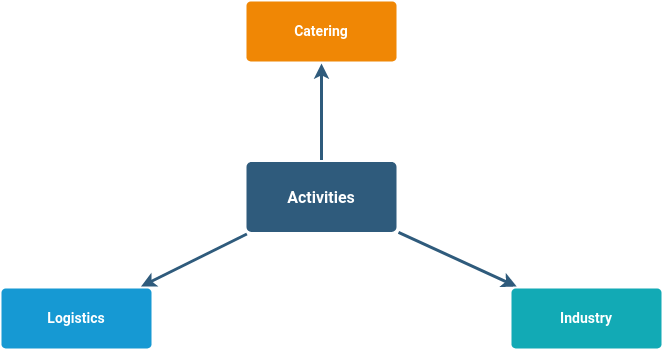
\includegraphics[width=0.8\textwidth]{images/core_activities.png}
\end{center}

Mainly handling the problems of management of part of the workflows in all these fields. 
And lately turning all their focus to logistics as their field of interest.

\begin{center}
    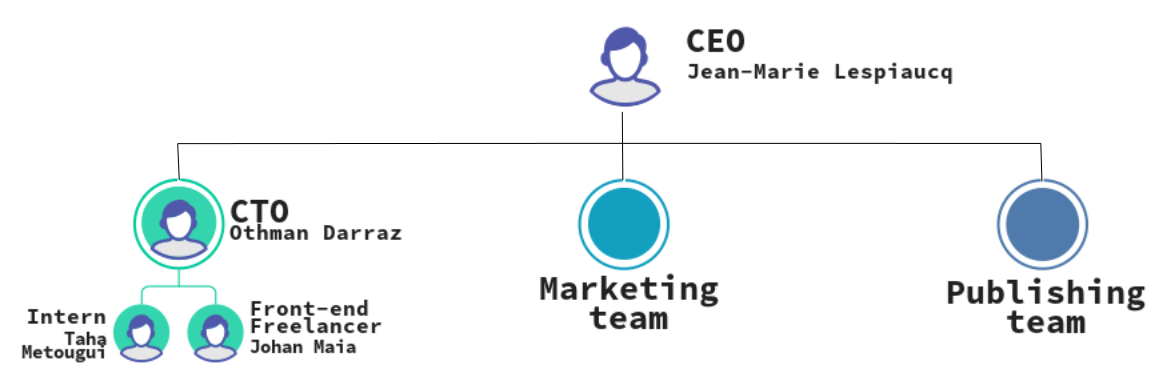
\includegraphics[width=0.85\textwidth]{images/Hierarchy}
\end{center}

The team, I've integrated, is composed of a team of 2 people, the CTO Othman Darraz who's in charge of managing the project
and a freelancer Johan who's in charge of everything that's front related, and me joining them as the third
member of the team taking care of backend mainly refactoring, optimization and security.




    \newpage

    \section{Assessment of current state}\label{sec:assessment-of-current-state}
    \subsection{Analysis}\label{subsec:analysis}
    Having to take care of managing multiple trucks, truck drivers, their turns, their parking lots
and their parking spaces can be a difficult task to achieve, especially when you have to deal with
time management, availability, delays, and so on.
However, going by old systems, either an Excel spreadsheet or just a ledger system on
paper, can help such a task, as long as you're working on a small scale. But once
this scales, the need for assistance grows.

And that's the point where comes the possibility to make use of automated tasks to do the job.
Automating the management, making it easier to manage with as little human intervention
as possible.

As of the current time, there is already a solution put in place, which is a SaaS hosted
on AWS implementing an SOA architecture. The SaaS relies on various managed services
provided by AWS, such as EC2, S3, RDS, etc.

The MMSoft Saas is constituted of:
\begin{itemize}
    \item Four front-end services:
    \begin{itemize}
        \item Easy-truck-in (ETI) interface which is the main interface
        \item Driver application (Angular 11)
        \item Registration Tablet App (React 16)
        \item Gatekeeper App (Cermate)
    \end{itemize}
    \item Four Back-end services:
    \begin{itemize}
        \item MQTT Broker communicating with the Gatekeeper app (VerneMQ)
        \item Orchestration Back-end Service (Java 11 Spring Boot 2.6) used by the ETI interface
        \item Registration Service (Node JS 16) used by the Registration Tablet App
        \item TMS Registration Back-end which exposes REST API for integration (Java 11 Spring Boot 2.6)
    \end{itemize}
    \item Two databases:
    \begin{itemize}
        \item MySQL for users, site, configuration
        \item Redis as a database for Daily/Weekly data and for messaging communication with other services
    \end{itemize}
\end{itemize}


And it has the following backend service used, as shown in the figure below:

\begin{center}
    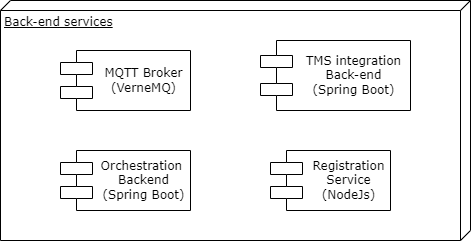
\includegraphics[width=0.8\textwidth]{images/Backend}
\end{center}





    \subsection{Criticism}\label{subsec:criticism}
    With the general structure of the software present, it is clear that the
software is missing some important features and building blocks that can make it 
the SaaS it's aimed to be.

To start with the essentials, as the software is targeted to be used for logistics
within factories and warehouses, it's important for the data of daily interactions and
operations to be stored in a database and be accessible to analytics and KPI's operations
to be able to provide a better understanding of their efficiency and how their
work is flowing. Because for the mean time, all the daily operations data is being stored
in the Redis database and Redis being an in-memory data structure store used as a database,
message broker, and streaming engine \cite{redis_def} it won't be suited for long term storage
as to keep it operational it will need to clear old data and free up space, thus why it's cleared
on a daily to weekly basis. And with no archival solution put in place, the data for now is
cleared then lost which means for any client opting to pull their old data for analytics
won't be possible.

Next comes the user management system, which is clearly a key factor in such a workflow, 
as seen in the \ref{fig:flowchart} there are multiple actors involved in the process,
from the gate keepers, operators, drivers, and the management staff. So with the current
user system which opts to have user set as a site which means for each factory there's a
single user or even though you can make multiple users they all will have full permission
in the site's scope which isn't secure neither is a good idea. So opting to a new system
which encourages the use of a role system for users and the users then belonging to a site
would be a better solution, as it would even open the flexibiltiy of adding configuration
to the user roles, and have each user have their own scope of permissions depending on
their role.

Also for the authentication, the current system uses a Bearer token which is a Json Web
Token (JWT) and that is permanent rather than an ephemeral one. So if an attacker manages
to intercept a token, which in fact is doable with code injections to expose a request,
then they can use it to access the backend at any time.
Opting to some other authentication system, such as a cookie based system, would be more
secure, as the cookies could at least be held in a secure place such as code injections,
can be used to acquire them from the front-end.

Looking at the current system and how the deployment is done, which is done in a manual way,
so it's takes more time to deploy simple bug fixes and new features reducing from the efficiency
of the developers, due to the time it takes to deploy each time. For fact, it's clear that
the addition of some automized deployment tools would be a good way reduce the need for the
manual deployment and also allow for faster deployment of new features and hot-fixes as the
deployment process is mostly a recurrent set of actions.

Next comes the code quality, which is rather messy, as it uses a lot of different tools,
some part are just redundant which could be done in a DRY\footnote{DRY or don't repeat
yourself is a term used to describe the practice of writing code that is not repetitive.
It is a way to reduce the amount of code that needs to be written.\cite{pragmatic_bro}} way,
not to the extreme of course where the code is becoming DRY but in expense of readability
and complexity. Other than the redundancy of some parts, the use of different approaches
in the code can get kind of messy and hard to maintain, especially if you're not familiar
with the code which would be the case in the expansion of the team, so the more the code
is unified the better. Also the code is not documented, so it's not clear what some parts
of the code internals do when it's something complex and that requires a modification.
The tests for the majority of the code are not put in place, so in the case of huge update
to the code, it would not be possible if some behaviour changed or if some parts are just 
not working.

There's the usage of different tech stacks which are NodeJS and Java Spring, which is a bit
of a mess, as it's not clear why the NodeJS is being used in the backend without much impact
as it's just handling some simple backend logic that could migrated to a Java Virtual
Machine(JVM)\footnote{JVM is the virtual machine that's capable of running Java binary
code}, compatible language such as Java, Kotlin, Scala, \dots, why I said a JVM compatible
language it's because the majority of the system is built on Java so it would make it
easier to migrate Js to Java than let's say moving the Java to NodeJS, but also to gain
the advantages of strongly typed language making it easier to pick up bugs. With such a
move, it would create a more uniform and rigid way to have the whole project fully handled
with single build tool, which in turn can really ease up the deployment process, and make
it automatable more easily.

One other point to tackle is security within the code, the current code base uses secrets
which are stored directly in the code, which is not secure, as you can easily acquire the
original code through a decompiling tool, or even through a reverse engineering tools,
which would make those secrets attainable directly. Opting for some other way of storing
the secrets, such as a database in addition with environment variables, would probably be
a better solution, in addition with a rolling system of secrets in possible cases making
those keys temporary.

\section{Conclusion}

To summarize the current state of the software, it's clear that the current application
is at in terms of the features and the current state of the code, it's clear that there's
a strong foundation for the application to be a SaaS as it's already handling almost the
full workflow of the fleet management system, , but there are some missing features and
building blocks specifically in the infrastructure and security aspects, which could be
mediated to complete the organization view of their product.


    \subsection{Proposed solution}\label{subsec:solution}
    


    \newpage

    \section{Business process}\label{sec:business-process}
    So for the business process, as stated previously, we have a set of activities that organizes the trucks and their drivers.
In the goal of have them work rather optimally in an automated fashion.

And it goes as follows:

\begin{center}
    \includegraphics[width=0.8\textwidth]{images/flowchart}
\end{center}

As seen in the diagram, it is rather a simple flowchart, but that would require to have a lot real time data put in place,
to have it coordinate with the trucks and drivers, without any downtimes.
And to adapt to the needs in hand, they've put in place the following IT infrastructure:

\begin{center}
    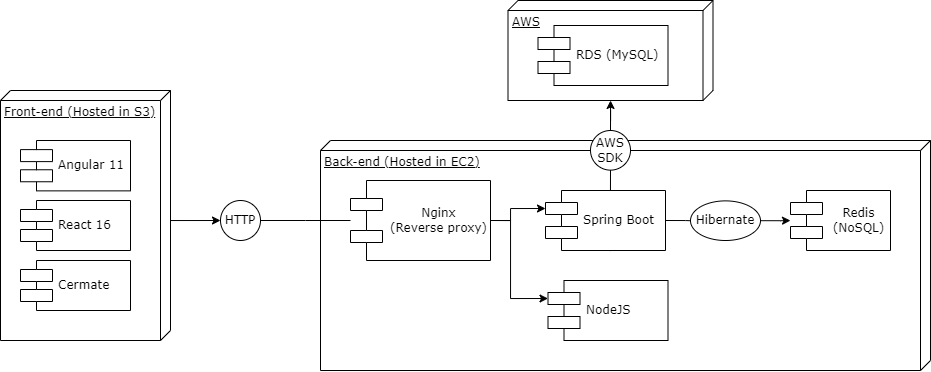
\includegraphics[width=0.8\textwidth]{images/State-of-art}
\end{center}

There are a lot of things that can be done to improve the performance of the system, but the main thing is to have a
base for the proof of concept.
As such, the released IT infrastructure is a good starting point for the proof of concept.

    \newpage

    \section{Conceptual model}\label{sec:conceptual-model}
    As of now the software is still in it very early stage, and being used mainly as a proof of concept.
And it's following the architecture below:

% TODO: this needs to get reworked
\begin{figure}[!htbp]
    \centering
    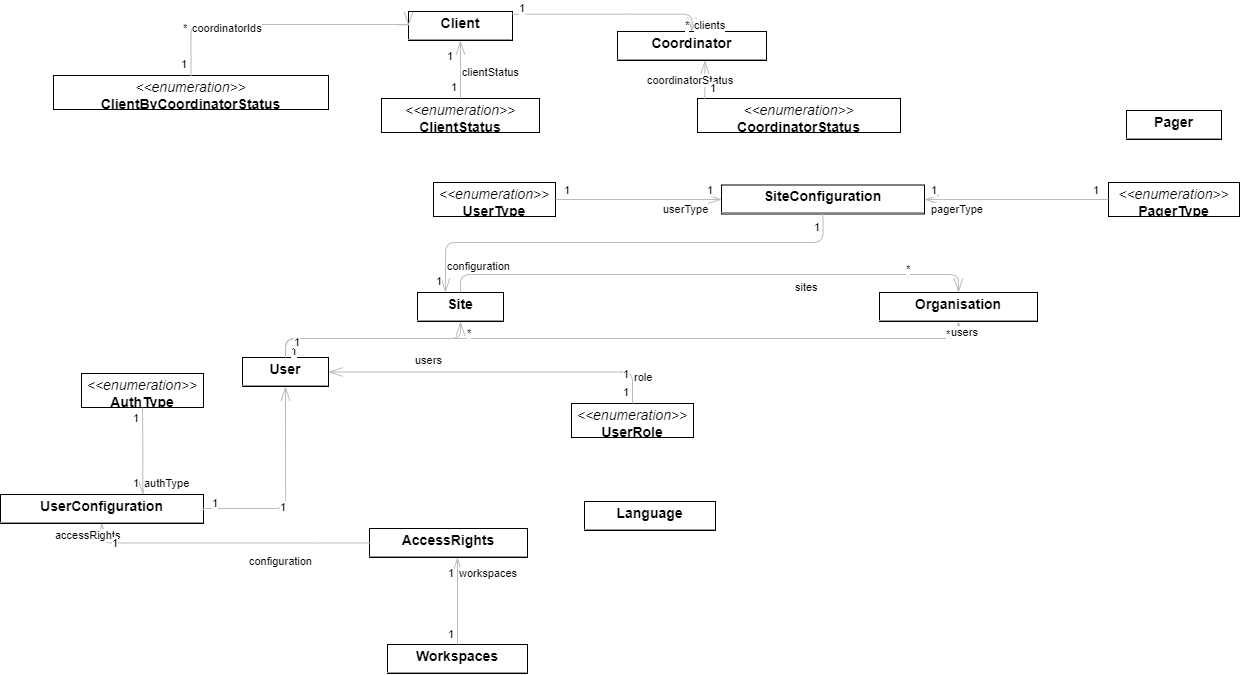
\includegraphics[width=1\textwidth]{images/package.drawio}
    \caption{\footnotesize{Backend model}}
    \label{fig:backend}
\end{figure}

% TODO: This part will be updated once we take on the subject of refactoring.



    \section{Target component Diagram}\label{sec:target-comp}
    As of the current moment the forecast component diagram for the system is as follows:

\begin{center}
    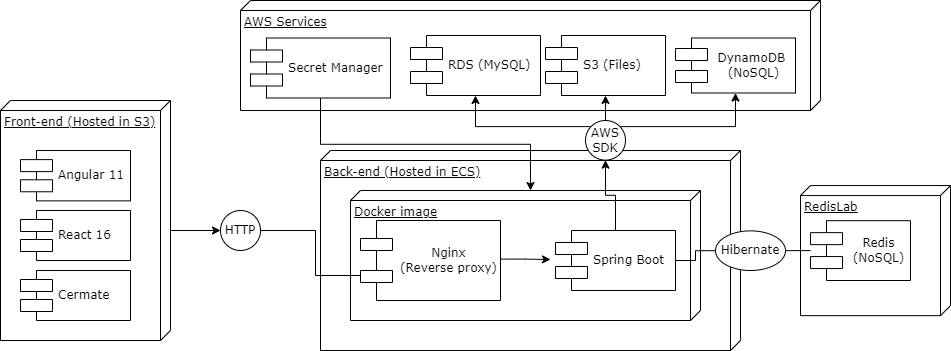
\includegraphics[width=0.8\textwidth]{images/forecast}
\end{center}

As it shows there are additional databases mainly ones for archiving files as is the case of
S3 and also archiving data for statistics down the line thus using DynamoDB\@.
Also containerizing the backend for the goal of having it run different instances seamlessly,
and have the run times duplicate efficiently.
For the creation of the images, it should be noted that they will be generated automatically,
and upload to ECR directly through CircleCI pipelines.
Thus the process of having to update or fix bugs within the back-end will be more streamlined
in a fashion that causes little to no downtime.


    \newpage

    \section{Implementation}\label{sec:implementation}

    \newpage

    \section{Conclusion}\label{sec:conclusion}

    \newpage

    \section{Appendices}\label{sec:appendices}

    \newpage

    \section{Bibliography}\label{sec:bibliography}

    \bibliography{main}
    \bibliographystyle{plain}

\end{document}
